\documentclass{article}
\usepackage[utf8]{inputenc}
\usepackage{graphicx}
\usepackage{subcaption} % Für \begin{subfigure}

\begin{document}

\begin{figure}
    \centering
    \begin{subfigure}[b]{0.3\textwidth}
        \centering
        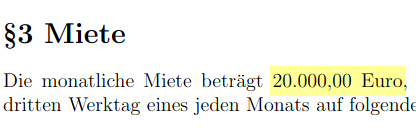
\includegraphics[width=\textwidth]{img/miete_chg.png}
        \caption{$y = x$}
        \label{fig:y_equals_x}
    \end{subfigure}
    \hfill
    \begin{subfigure}[b]{0.3\textwidth}
        \centering
        \includegraphics[width=\textwidth]{example-image-b}
        \caption{$y = 3\sin x$}
        \label{fig:three_sin_x}
    \end{subfigure}
    \hfill
    \begin{subfigure}[b]{0.3\textwidth}
        \centering
        \includegraphics[width=\textwidth]{example-image-c}
        \caption{$y = \frac{5}{x}$}
        \label{fig:five_over_x}
    \end{subfigure}
    \caption{Three simple graphs}
    \label{fig:three_graphs}
\end{figure}

\end{document}